\documentclass[]{article}
\title{CS3.301 - Assignment 1}
\author{Emmanuel Roshan Jaiby, 2025101010}
\date{}
\usepackage{enumitem} % used for itemize
\usepackage{tikz}
\usetikzlibrary{automata, positioning, arrows.meta} % used for automata diagrams
\usepackage{amssymb}
\usepackage[]{amsmath} % used for matrices, Q6
\begin{document}
	\maketitle
	
	\section*{Q1.}
	(a) Let $\Sigma = \{a, b\}$. For each $k \geq 1$, let $C_{k}$ be the language consisting of all strings that contain an $a$ exactly $k$ places from the right-hand end. Describe an NFA with $k+1$ states that recognizes $C_{k}$, both in terms of a state diagram and a formal description.  \\
	(b) Consider the languages $C_k$ defined in the previous problem. Prove that for each $k$, no DFA can recognize $C_k$ with fewer than $2^{k}$ states.
	\paragraph{Sol.} Let $M_k$ be the NFA recognising $C_k$. Then $ M_k $ is given by the 5-tuple $(Q, \Sigma, \delta, q_0, F)$, where:
	\begin{itemize}[label={}, noitemsep]
		\item $Q = \{q_0, \cdots, q_k\}$,
		\item $\Sigma = \{a, b\}$,
		\item $q_0 \in Q$ is the start state,
		\item $F = \{q_k\}$,
	\end{itemize} 
	and $ \delta : Q \times \Sigma \rightarrow \mathcal{P}(Q) $ is given by:
	\begin{itemize}[label={}, noitemsep]
		\item $ \delta(q_0, a) = \{q_0, q_1\} $
		\item $ \delta(q_0, b) = \{q_0\} $
		\item $ \delta(q_i, a) = \{q_{i+1}\} $ for all $ 1 \leq i \leq k - 1 $ and $k \geq 2$
		\item $ \delta(q_i, b) = \{q_{i+1}\} $ for all $ 1 \leq i \leq k - 1 $ and $k \geq 2$
	\end{itemize}
	This NFA loops at $q_0$ until it guesses non-deterministically when it reads an $a$ that it is $k$ places from the right-hand end. It then transitions to $q_1$. All further states simply serve to count the $k$ places from the right-hand end. 
	\begin{figure}[h]
		\centering
		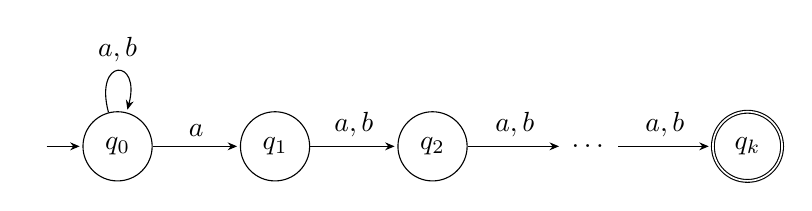
\begin{tikzpicture}[shorten >=1pt, node distance=2cm, on grid, 	auto, >={Stealth[length=1.2mm, width=1mm]}]
			\node[state, initial, initial text=] (q0) {$q_0$};
			\node[state] (q1) [right=of q0] {$q_1$};
			\node[state] (q2) [right=of q1] {$q_2$};
			\node[draw=none] (dots) [right=of q2] {$\dots$};
			\node[state, accepting] (qk) [right=of dots] {$q_k$};
			\path[->] 
			(q0) edge [loop above] node {$a, b$} (q0)
			(q0) edge node {$a$} (q1)
			(q1) edge node {$a, b$} (q2)
			(q2) edge node {$a, b$} (dots)
			(dots) edge node {$a, b$} (qk);
		\end{tikzpicture}
		\caption{NFA $M_k$ recognizing $C_k$.}
	\end{figure}
	\\ \\
	\subparagraph{}Intuitively, a DFA that recognizes $C_k$ must be able to "remember" the last $k$ symbols. Since there are $2^k$ such strings, if the DFA has fewer than $2^k$ states, then there would be some state $q$ that can be reached by two different strings of length $k$. \subparagraph{} Let these two strings be $x$ and $y$. \subparagraph{Case 1.} If they differ at the first position, then one of them must start with a 0 and one must start with a 1. By symmetry, let $x$ start with a 0 and $y$ start with a 1.  \\Then, $x$ is a string that does not have a 1 $k$ places from the right-hand end, and hence $q \not\in F$. However, $y$ is a string that has a 1 $k$ places from the right-hand end and hence $q \in F$. This is a contradiction. \subparagraph{Case 2.} If they differ at some position $i \neq 1$, then suffix both $x$ and $y$ with $i-1$ zeroes. Now, one can take the suffixes $x'$ and $y'$ of length $k$ of $x$ and $y$ respectively. $x'$ and $y'$ differ at the first position and lead to the same state $q$. Now, by the argument in the previous case, there is a contradiction. \subparagraph{} Hence, a DFA recognizing $C_k$ must have $2^k$ states. $ \blacksquare $
	\pagebreak
	\section*{Q2.}
	The Hamming distance between two words of equal length is the number of positions at which they differ. Prove that for every regular language $L$ and every constant $k$, the set of words at a distance at most $k$ from a word in $L$ is regular.
	
	\paragraph{Sol.}  Since $L$ is regular, there is a DFA $M$ that recognizes it, given by $(Q, \Sigma, \delta, q_0, F)$. We construct an NFA $M_k$ that recognises the language of all strings that are at a distance of at most $k$ from any word in $L$ as $$(Q \times \{0, 1, \dots, k\}, \Sigma, \delta_k, (q_0, 0), F \times \{0, 1, \dots, k\})$$ and $ \delta_k : Q \times \{0, 1, \dots, k\} \times \Sigma \rightarrow \mathcal{P}(Q \times \{0, 1, \dots, k\})$ is given by:
	$$\delta_k((q, i), a) = \{(\delta(q,a), i)\} \cup \{(\delta(q, b), i+1):b \in \Sigma \setminus \{a\}\} \quad  i < k$$
	$$\delta_k((q, k), a) = \{(\delta(q,a), k)\} \cup \emptyset $$
	\subparagraph{}$M_k$ non-deterministically guesses whether the character it reads is correct or wrong. The correct case corresponds to $\{(\delta(q, a), i)\}$ and the wrong case corresponds to the set of states with the error counter $i$ incremented and all other characters considered to be possibly right. When $k$ errors have accumulated and $M_k$ guesses the character read is "wrong", it enters a dead state $\emptyset$.
	\subparagraph{} If the input string has no errors, since it would have reached a state $q \in F$ in the original DFA $M$, it will reach $(q,0)$ on at least one run, and hence be accepted. \subparagraph{} If the input string has no more than $k$ errors, on at least one run, $M_k$ at every error will guess the "correct" character in its place, and reach an accepting state $(q, n)$, where $n \leq k$. \subparagraph{} If the input string has more than $k$ errors, then $M_k$, after recognising and correcting the first $k$ errors on all runs, must send it to the dead state on the $(k+1)\textsuperscript{th}$ error or assume it is correct and then fail or crash.
	
	$\blacksquare$
	\pagebreak
	\section*{Q3.}
	Minimize the DFA given below.
	\paragraph{Sol.}
		\begin{figure}[]
			\centering
			\begin{tikzpicture}[
				shorten >=1pt, node distance=2.2cm,	on grid,
				auto, very thin, >={Stealth[length=1.2mm, width=1mm]}
				]
				\node[state, initial, initial text=] (0) {$0$};
				\node[state] (1) [below=1.6cm of 0] {$1$};
				\node[state, accepting] (2) [right=3.2cm of 1] {$2$};
				\node[state] (3) [right=3.2cm of 2] {$3$};
				\node[state] (5) [below=2cm of 2] {$5$};
				\node[state] (7) [below=1.4cm of 5] {$7$};
				\node[state] (4) [below left=1.8cm and 2.6cm of 5] {$4$};
				\node[state] (6) [below right=1.8cm and 2.6cm of 5] {$6$};
				\path[->] 
				(0) edge node [left] {$0$} (1)
				(0) edge [out=210, in=180, looseness=1.5] node [below left] {$1$} (5)
				(1) edge node [above] {$1$} (2)
				(1) edge [out=60, in=60, looseness=2.3] node [above, pos=0.5] {$0$} (6)
				(2) edge [loop above] node {$1$} (2)
				(2) edge node [above left] {$0$} (0)
				(3) edge node [above] {$0$} (2)
				(3) edge node [right] {$1$} (6)
				(4) edge node [above left] {$1$} (5)
				(4) edge node [above left] {$0$} (7)
				(5) edge node [left] {$0$} (2)
				(5) edge node [above right] {$1$} (6)
				(6) edge [out=300, in=330, loop] node [above right] {$0$} (6)
				(6) edge node [bend left, below] {$1$} (4)
				(7) edge [out=45, in=315] node [right] {$1$} (2)
				(7) edge node [above] {$0$} (6);
			\end{tikzpicture}
			\caption{DFA}
		\end{figure}
	We first eliminate all states unreachable from the start state, i.e., state 3.
	We then separate the remaining states into two groups \textemdash accepting and non-accepting states.
	$$\{0, 1, 4, 5, 6, 7\} \{ 2 \}$$
	These states, upon reading 0, go to the following respectively:
	$$\{1, 6, 7, 2, 6, 6\} \{1\} $$
	Since state 5 on a read of 0 is accepting and the states 0, 1, 4, 6, 7 are not, state 5 is distinguished from them.
	$$\{0, 1, 4, 6, 7\} \{2\} \{5\}$$
	These states, upon reading 1, go to the following respectively;
	$$\{5, 2, 5, 4, 2\} \{2\} \{6\}$$
	Depending on which group they go to, the pair of states $(0,4)$ and $(1, 7)$ are distinguished from each other.
	$$\{0, 4\} \{1, 7\} \{2\} \{5\} \{6\} $$
	The pair $(1, 7)$ are indistinguishable since they go to states 2 and 6 upon reading 1 and 0, respectively.
	The pair $(0, 4)$ are indistinguishable since, upon reading 0, they go to $(1,7)$ respectively, which is an indistinguishable pair, and upon reading 1, they both go to state 5.
	Hence, the minimal DFA is given by the following:
	\begin{figure}[]
		\centering
		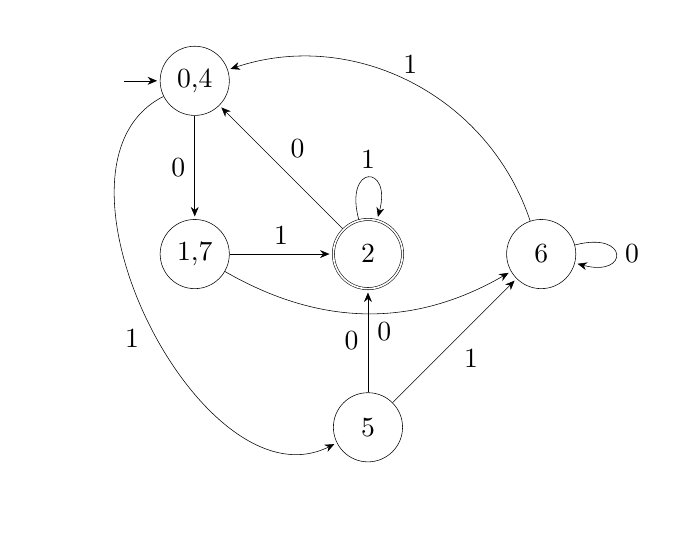
\begin{tikzpicture}[
			shorten >=1pt, node distance=2.2cm,	on grid,
			auto, very thin, >={Stealth[length=1.2mm, width=1mm]}
			]
			\node[state, initial, initial text=] (04) {0,4};
			\node[state] (17) [below=of 04] {1,7};
			\node[state, accepting] (2) [right=of 17] {2};
			\node[state] (5) [below=of 2] {5};
			\node[state] (6) [right=of 2] {6};
			\path[->] 
			(04) edge node [left] {$0$} (17)
			(04) edge [bend right=90] node [below left] {$1$} (5)
			(17) edge node [above] {$1$} (2)
			(17) edge [bend right=30] node [below right] {$0$} (6)
			(2) edge [loop above] node {$1$} (2)
			(2) edge node [above right] {$0$} (04)
			(5) edge node [left] {$0$} (2)
			(5) edge node [below right] {$1$} (6)
			(6) edge [loop right] node {$0$} (6)
			(6) edge [bend right=45] node [above] {$1$} (04);
		\end{tikzpicture}
		\caption{Minimised DFA}
	\end{figure}
	\pagebreak
	\section*{Q4.}
	Let $\Sigma = \{a\}$ be a single-letter alphabet. Prove that a language $L \subseteq \Sigma^*$ is regular if and only if the set of the lengths of its words, $S = \{|w| | w \in L\}$, is ultimately periodic. \\
	\textbf{Def.} A set of natural numbers $S \subseteq \mathbb{N}$ is ultimately periodic if there exists a threshold integer $N \geq 0$ and a period integer $p \geq 1$ such that for all integers $n \geq N$:
	$$ n \in S \iff n + p \in S $$ 
	
	\paragraph{Sol.}  
	\subparagraph{Forward Direction.} Let the lengths of words of $L$ be ultimately periodic. Then, there exists a threshold integer $N \geq 0$ and a period integer $p \geq 1$. Then, L is a union of regular languages given by: $$L = \{a^n | n \in S, n < N\} \cup \bigcup_{i \in I} \{a^{N+i+kp} | k \geq 0\}$$ where $I = \{i \in \{0,1, \dots, p-1 \}| N+i \in S\}$ and is hence itself finite under closure of finite union, since the first term in the union is a finite language and the second is represented as a union of regular languages $a^{N+i}(a^p)^*$.
	\subparagraph{Backward Direction.} Let $D$ be the DFA that recognizes $L$. Since $D$ is a finite automaton, it must have a finite number of states. 
	\subparagraph{} If $L$ is finite, then there is a maximum length $max(S)$. Let the threshold integer $N = max(S) + 1$ and the period integer $p = 1$. Then, $\forall n \geq N, n \in S \iff n + p \in S$ is vacuously true. Hence, the set of the lengths of the words of $L$ is ultimately periodic.
	\subparagraph{} If $L$ is infinite, then by the pigeonhole principle, there must be strings that end at the same state despite being of different lengths, since for any number of states of the DFA recognizing $L$, there must be strings of length greater than that number, since otherwise $L$ would be finite. Consider he sequence of states $q_0, q_1, \dots$ where $q_k = \hat{\delta}(q_0, a^k)$. By the pigeonhole principle, there are indices $m, m+p$ such that $q_m = q_{m+p}$. For integers $n \geq m$, $a^{n+p} = a^{m + p} a^{n-m} = a^m a^{n-m} = a^n.$ Since $\hat{\delta}(q_0, a^m) = q_m$ and $\hat{\delta} (q_m, a^p) = q_{m+p} = q_m$, $\hat{\delta}(q_0, a^{n+p}) = \hat{\delta}(q_0, a^n) = q_n$. Hence, $a^n \in L \iff q_n \in F \iff q_{n+p} \in F \iff a^{n+p} \in L$. Equivalently, $n \in S \iff n+p \in S$. $\blacksquare$
	\pagebreak
	\section*{Q5.}
	Consider the language $L=\{a^ib^j | i \neq j\}$. \\
	(a) Prove that $L$ is not regular using the pumping lemma. \\
	(b) Provide a much shorter proof that $L$ is not regular using only closure properties and the known non-regular language $\{a^nb^n | n \geq 0\}$.
	
	\paragraph{Sol.} 
	
	\subparagraph{a.} Assume to the contrary that $L$ is regular.
	Let $p$ be the pumping length given by the pumping lemma. Consider a string $w = a^p b^{p+p!} \in L$. Now, by the pumping lemma, we can break $w$ into three strings $xyz$ such that $y \neq \epsilon$, $|xy| \leq p$, and $\forall k \geq 0, xy^k z \in L$. The largest possible $xy$ is $a^p$. Choose $y = a^m, 1 \leq m \leq p$. Now, $\forall k \geq 0, xy^k z \in L$. Choose $k=1+\frac{p!}{m}. $ Then, $$xy^k z = a^{p+p!} b^{p+p!}$$, which is not in $L$. Hence, $L$ is non-regular. $\blacksquare$
	
	\subparagraph{b.}  Assume to the contrary that $L$ is regular. Let $R$ be the regular language described by the regular expression $a^*b^*$. $R$ is regular since both $a*$ and $b^*$ are regular languages by closure under the star operation and closure under the concatenation operation. Since $L$ is regular, by closure under complement, $\bar{L}$ is regular. $R \setminus L$ is regular since $R \setminus L = R \cap \bar{L} = \bar{\bar{R} \cup L}$ is closed under complementation and union. $R \setminus \bar{L}$ consists of those strings of zero or more $a$'s followed by zero or more $b$'s such that the number of $a$'s is not unequal to the number of $b$'s. Hence, $R \setminus L = \{0^n 1^n | n \geq 0\}$. But this is a contradiction since $\{0^n 1^n | n \geq 0\}$ is a non-regular language. Hence $L$ must be non-regular. $\blacksquare$
	
	\pagebreak
	
	\section*{Q6.}
	Let $$\Sigma_3 = \begin{Bmatrix} \begin{bmatrix} 0 \\ 0 \\ 0 \end{bmatrix},  \begin{bmatrix} 0 \\ 0 \\ 1 \end{bmatrix}, \begin{bmatrix} 0 \\ 1 \\ 0 \end{bmatrix}, \dots, \begin{bmatrix} 1 \\ 1 \\ 1 \end{bmatrix} \end{Bmatrix}.$$
	$\Sigma_3$ contains all size-3 columns of 0s and 1s. A string of symbols in $\Sigma_3$ gives three rows of 0s and 1s.	Consider each row to be a binary number written with the least significant bit first (i.e. the leftmost
	column is the units bit) and let
	$$ B = \{w \in \Sigma_3^{*} \enspace | \text{ the bottom row of } w \text{ is the sum of the top two rows} \}. $$
	For example,
	$$ \begin{bmatrix} 1 \\ 1 \\ 0 \end{bmatrix} \begin{bmatrix} 0 \\ 1 \\ 0 \end{bmatrix} \begin{bmatrix} 0 \\ 0 \\ 1 \end{bmatrix} \in B, \qquad \text{ but } \qquad \begin{bmatrix} 1 \\ 0 \\ 1 \end{bmatrix} \begin{bmatrix} 0 \\ 0 \\ 1 \end{bmatrix} \not\in B. $$
	Show that $B$ is regular.
	
	\paragraph{Sol.} We construct a DFA $D_B = (Q, \Sigma_3, \delta, q_0, F)$ to recognise the language $B$ by:
	\begin{itemize}[label={}, noitemsep]
		\item $Q = \{q_0, q_1, q_X\}$,
		\item $q_0 \in Q$ is the start state,
		\item $F = \{q_0\}$,
	\end{itemize} 
	and $\delta: Q \times \Sigma_3 \rightarrow Q$ is given by the transition diagram.
	\begin{figure}[]
		\centering
		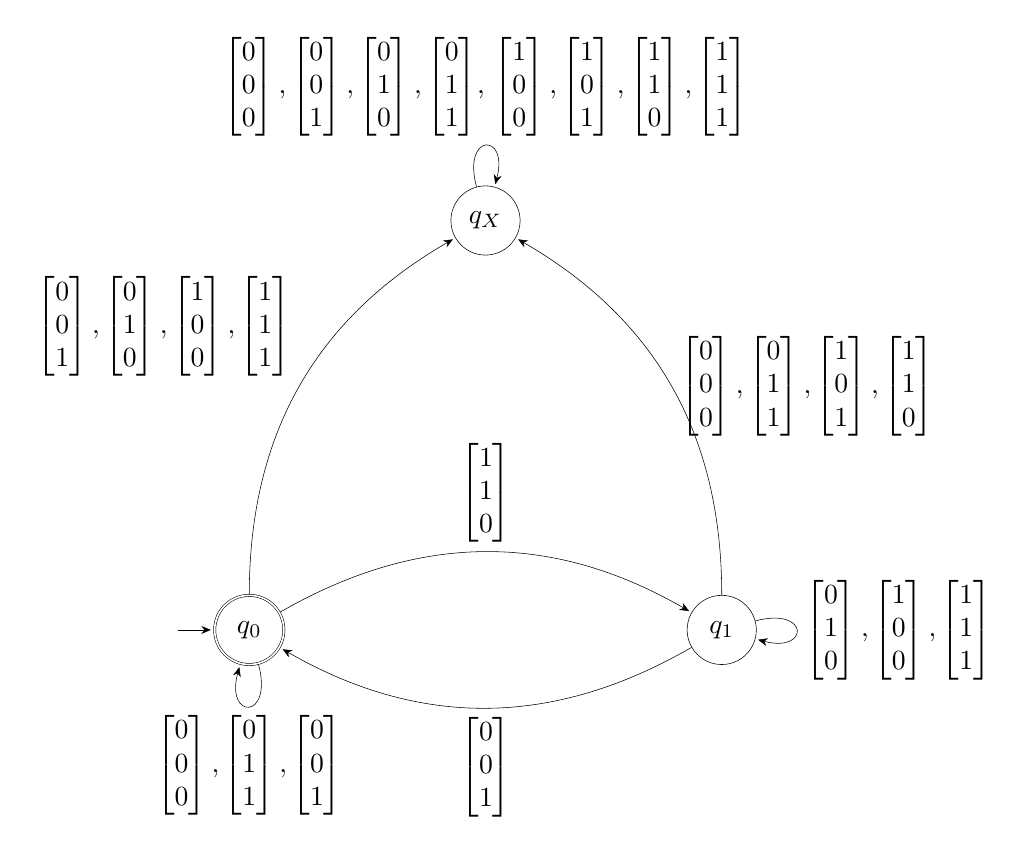
\begin{tikzpicture}[
			shorten >=1pt, node distance=2.2cm,	on grid,
			auto, very thin, >={Stealth[length=1.2mm, width=1mm]}
			]
			\node[state, initial, accepting, initial text=] (q_0) at (0, 0) {$q_0$};
			\node[state] (q_1) at (6,0)  {$q_1$};
			\node[state] (q_X) at (3, 5.2) {$q_X$};
			\path[->] 
			(q_0) edge [loop below] node {$\begin{bmatrix} 0 \\ 0 \\ 0 \end{bmatrix}, \begin{bmatrix} 0 \\ 1 \\ 1 \end{bmatrix} , \begin{bmatrix} 0 \\ 0 \\ 1 \end{bmatrix}$} (q_0)
			(q_0) edge [bend left] node {$\begin{bmatrix} 1 \\ 1 \\ 0 \end{bmatrix}$} (q_1)
			(q_1) edge [bend left] node {$\begin{bmatrix} 0 \\ 0 \\ 1 \end{bmatrix}$} (q_0)
			(q_1) edge [loop right] node {$\begin{bmatrix} 0 \\ 1 \\ 0 \end{bmatrix}, \begin{bmatrix} 1 \\ 0 \\ 0 \end{bmatrix} , \begin{bmatrix} 1 \\ 1 \\ 1 \end{bmatrix}$} (q_1)
			(q_0) edge [bend left] node {$\begin{bmatrix} 0 \\ 0  \\ 1 \end{bmatrix}, \begin{bmatrix} 0 \\ 1  \\ 0 \end{bmatrix}, \begin{bmatrix} 1 \\ 0  \\ 0 \end{bmatrix}, \begin{bmatrix} 1 \\ 1  \\ 1 \end{bmatrix}$} (q_X)
			(q_1) edge [bend right] node [right] {$\begin{bmatrix} 0 \\ 0  \\ 0 \end{bmatrix}, \begin{bmatrix} 0 \\ 1  \\ 1 \end{bmatrix}, \begin{bmatrix} 1 \\ 0  \\ 1 \end{bmatrix}, \begin{bmatrix} 1 \\ 1  \\ 0 \end{bmatrix}$} (q_X)
			(q_X) edge [loop above] node {$\begin{bmatrix} 0 \\ 0  \\ 0 \end{bmatrix}, \begin{bmatrix} 0 \\ 0  \\ 1 \end{bmatrix}, \begin{bmatrix} 0 \\ 1  \\ 0 \end{bmatrix}, \begin{bmatrix} 0 \\ 1  \\ 1 \end{bmatrix}$, $\begin{bmatrix} 1 \\ 0  \\ 0 \end{bmatrix}, \begin{bmatrix} 1 \\ 0  \\ 1 \end{bmatrix}, \begin{bmatrix} 1 \\ 1  \\ 0 \end{bmatrix}, \begin{bmatrix} 1 \\ 1  \\ 1 \end{bmatrix}$} (q_X);
		\end{tikzpicture}
		\caption{Transition diagram for $\delta$}
	\end{figure}
	The dead state $q_X$ is transitioned to when the input string, no matter the suffix, cannot possibly be in $B$. $q_0$ represents a valid string in $B$ with carry 0, and $q_1$ represents a valid string satisfying the property that the last row is the sum of the first two that has a carry of 1. If, in $q_0$, despite having no carry, a symbol is read that would require carry 1 to be valid, or vice-versa in $q_1$, it is to $q_X$ that a transition occurs.
	
	\pagebreak
	
	\section*{Q7.}
	Prove that the following languages are not regular: \\
	(a) $\{a^{2^n} : n \in \mathbb{N}\}$ \\
	(b) $\{a^p : p \text{ is a prime number.}\}$ \\
	(c) $\{a^i b^j : \gcd{(i, j)} = 1\}$ \\
	(d) $\{\text{bin}(p) : p \text{ is a prime number.}\}$ \\
	
	\paragraph{Sol.}
	\subparagraph{a.} Assume, to the contrary, that $L = \{a^{2^n} : n \in \mathbb{N}\}$. Let $p$ be the pumping length specified by the pumping lemma. Consider the string $a^{2^p} \in L$. Since $a^{2^p}$ is composed solely of $a$'s, $xy = a^p$. Let $y = a^m$, where $1 \leq m \leq p$. By the pumping lemma, all strings of the form $xy^i z \in L$. Let $i = 2$. Then, $xy^2z = a^{2^p + m}$. $2^p < 2^p + 1 \leq 2^p + m \leq 2^p + p < 2^{p+1}$, since $2^x > x \forall x \in \mathbb{R}$. Hence, $2^p + m$ is between two consecutive powers of two and cannot be a power of two. This is a contradiction, Hence, $L$ is non-regular. $\blacksquare$
	\subparagraph{b.} Assume, to the contrary, that $L = \{a^p : p \text{ is a prime number.}\}$ is a regular language. Let $q$ be the pumping length specified by the pumping lemma. Consider the string $a^n$, where $n$ is the smallest prime strictly greater than $q$. Now, the pumping lemma states that $a^n$ can be split into three strings $xyz$ such that $$xyz = a^n,|y| > 0, |xy| \leq q, xy^i z \in L \quad \forall i \geq 0$$. Let $|y| = m > 0$ and $i = n+1$. Then, $xy^iz = a^{n+nm}$. $n+nm = n(1+m)$, which is composite. Hence, $xy^iz \not\in L$. This is a contradiction. Hence, $L$ is non-regular. $\blacksquare$
	\subparagraph{c.} Assume, to the contrary, that $L = \{a^i b^j : \gcd(i,j) = 1\}$ is a regular language. Let $p$ be the pumping length specified by the pumping lemma. Consider the string $a^{q-1} b^q$, where $q$ is a prime strictly greater than $2p$, which is in $L$ since $p$ has only $1$ and $q$ as factors, and since $(-1)(q-1) + (1)q = 1$, by Bézout's lemma, $\gcd(q-1, q) = 1$.
	Now, the pumping lemma states that $a^n$ can be split into C. Let $|y| = m$. Since $q$ is prime, by Bézout's lemma, $ \exists s, t \in \mathbb{Z} \text{ s.t. } sm+tq =  \gcd(m,q) = 1$, since $m \leq p < q$. Let $r$ be the smallest integer such that $s + rq > 0$. Let $i = 1+s+rq$. Then, $xy^i z = a^{p-m} (a^m)^{1+s+rq} a^{q-p-1} b^q = a^{q-1+m(s+rq)} b^q$. Now, $q-1+m(s+rq) = -1 + 1 + 0 (\mod q)$, since $ms = 1-tq \equiv 1 (\mod q)$. So $q \mid q-1+m(s+rq)$ and hence $\gcd(q, q-1+m(s+rq)) \neq 1$. This is a contradiction. Hence $L$ is non-regular. $\blacksquare$
	\subparagraph{d.} Assume, to the contrary, that $L = \{\text{bin} (p) : p \text{ is a prime number,} \}$ is regular. Then, there is a DFA $D$ that recognizes $L$. Then, let $k$ be the number of states in $D$. Then, $k$ is also the pumping length specified by the pumping lemma. Let $p$ be a prime whose binary representation has more than $k$ digits. Let $\text{bin}(p)$ be split into three strings $xyz$ per the pumping lemma. Let $p_i$ be the value of the pumped string $xy^i z$. $$p_i = \text{val}(x) 2^{im + n} + \text{val}(y) 2^n (1+ 2^m + 2^{2m} + \dots +  2^{(i-1)m}) + \text{val}(z)$$
	Hence, $$p_i = \text{val}(x) 2^{im + n} + \text{val}(y) 2^n \frac{2^{im} - 1}{2^m - 1} + \text{val}(z)$$. Since $p = p_1$ is odd (since if $D$ had only one state, only then would $p$ possibly equal two, but then $D$ must accept all inputs or reject all inputs, and it would not then recognize $L$, hence it must have at least two states, i.e., $p$ is at least 5), $\gcd{2,j} = 1$. Hence, by Fermat's little theorem, $2^{p-1} \equiv 1 (\mod p)$. Consider $$p_p = \text{val}(x) 2^{pm + n} + \text{val}(y) 2^n \frac{2^{pm} - 1}{2^m - 1} + \text{val}(z) \equiv \text{val}(x) 2^{m+n} + \text{val}(y) 2^n + \text{val}(z) \equiv p \equiv 0 (\mod p)$$, since $2^{pn} = 2^{n + (p-1)n} = 2^n (2^n)^{p-1} \equiv 2^n (1) (\mod p)$. Hence, the pumped string is composite. This contradicts the assumption that $L$ is regular. Hence, $L$ is non-regular. $\blacksquare$.
	\pagebreak
	\section*{Q8.}
	Prove that the following grammars are ambiguous by providing a string with two
	different leftmost/rightmost derivations, or two different parse trees: \\
	(a) $$ S \rightarrow aAB $$ $$ A \rightarrow bBb $$ $$B \rightarrow A | \lambda $$ \\
	(b) $$ S \rightarrow SS | \lambda | aSb | bSa $$ \\
	(c) $$ S \rightarrow aSb | SS | \lambda $$
	
	\paragraph{Sol.} 
	\subparagraph{a.} Consider the string $abbbb$.
	\subparagraph{Derivation 1.}
	$S \rightarrow aAB$ \\ $ aAB \rightarrow abBbA $ (by $A \rightarrow bBb$) \\ $abBbA \rightarrow abbA$ (by $B \rightarrow \lambda$) \\ $abbA \rightarrow abbbBb$ (by $A \rightarrow bBb$) \\ $abbbBb \rightarrow abbbb$ (by $B \rightarrow \lambda$)
	\subparagraph{Derivation 2.}
	$S \rightarrow aAB$ \\ $ aAB \rightarrow abBb $ (by $A \rightarrow bBb$) \\ $abBb \rightarrow abAb$ (by $B \rightarrow A$) \\ $abAb \rightarrow abbBbb$ (by $A \rightarrow bBb$) \\ $abbBbb \rightarrow abbbb$ (by $B \rightarrow \lambda$). \\
	Since there are 2 leftmost derivations of the string $abbbb$, the CFG is ambiguous. $\blacksquare$
	\subparagraph{b.} Consider the string $ab$.
	\subparagraph{Derivation 1.} 
	$ S \rightarrow SS$ \\ $ SS \rightarrow aSbS$ (by $S \rightarrow aSb$) \\ $ aSbS \rightarrow abS$ (by $S \rightarrow \lambda$) \\ $abS \rightarrow ab$ (by $S \rightarrow \lambda$).
	\subparagraph{Derivation 2.}
	$ S \rightarrow aSb $ \\ $ aSb \rightarrow ab $ (by $S \rightarrow \lambda$). \\
	Since there are 2 leftmost derivations of the string $ab$, the CFG is ambiguous. $\blacksquare$
	\subparagraph{c.} Consider the string $ab$.
	 \subparagraph{Derivation 1.} 
	 $ S \rightarrow SS$ \\ $ SS \rightarrow aSbS$ (by $S \rightarrow aSb$) \\ $ aSbS \rightarrow abS$ (by $S \rightarrow \lambda$) \\ $abS \rightarrow ab$ (by $S \rightarrow \lambda$).
	 \subparagraph{Derivation 2.}
	 $ S \rightarrow aSb $ \\ $ aSb \rightarrow ab $ (by $S \rightarrow \lambda$). \\
	Since there are 2 leftmost derivations of the string $ab$, the CFG is ambiguous. $\blacksquare$
	\pagebreak
	\section*{Q9.}
	Construct a PDA for each of the following languages. \\
	(a) $$ L = \{a^m b^n | m \leq n \leq 2m\}$$. \\
	(b) $$ L = \{a^i b^j c^k | i = j \text{ or } j = k\}$$. \\
	(c) For any one of the above parts, if you constructed a PDA which accepts by final state, convert it into a PDA which accepts by empty stack instead; and vice-versa if you did it the other way around.
	\paragraph{Sol.}
	\subparagraph{a.}
	Let $M$ be the PDA given by $(Q, \Sigma, \Gamma, \delta, q_0, F)$ where:
	\begin{itemize}[label={}, noitemsep]
		\item $Q = \{q_a, q_1, q_b, q_f\}$
		\item $\Sigma = \{a, b\}$
		\item $\Gamma = \{X\}$
		\item $F = \{q_f\}$
	\end{itemize}
	and $\delta: Q \times \Sigma_\epsilon \times \Gamma_\epsilon \rightarrow \mathcal{P}(Q \times \Gamma_\epsilon)$ is given by: 
	\begin{itemize}[label={}, noitemsep]
		\item $\delta(q_0, a, \epsilon) \rightarrow \{(q_0, a), (q_1, a)\}$
		\item $\delta(q_1, \epsilon, \epsilon) \rightarrow \{(q_0, a)\}$
		\item $\delta(q_0, \epsilon, \$) \rightarrow \{(q_f, \$)\}$
		\item $\delta(q_0, b, a) \rightarrow \{(q_1, \epsilon)\}$
		\item $\delta(q_1, b, a) \rightarrow \{(q_1, \epsilon)\}$
		\item $\delta(q_1, \epsilon, \$) \rightarrow \{(q_f, \$)\}$
	\end{itemize}
	and we assume $\$$ is on the stack before execution starts.
	While reading $a$'s, $M$ pushes one or two $a$'s onto the stack, non-deterministically. When it reads $b$'s, it pops one off the stack. If the string is empty, i.e., $m = n = 0$, or when the end of the input string is reached, if $M$ is in the final state $q_f$, it accepts, if the stack marker $\$$ is on top to signal it is effectively empty.
	\subparagraph{b.}
	LLet $M$ be the PDA given by $(Q, \Sigma, \Gamma, \delta, q_0, F)$ where:
	\begin{itemize}[label={}, noitemsep]
		\item $Q = \{q_0, q_{1a}, q_{1b}, q_{1c}, q_{2a}, q_{2b}, q_{2c}, q_f\}$
		\item $\Sigma = \{a, b, c\}$
		\item $\Gamma = \{X\}$
		\item $F = \{q_f\}$
	\end{itemize}
	and $\delta: Q \times \Sigma_\epsilon \times \Gamma_\epsilon \rightarrow \mathcal{P}(Q \times \Gamma_\epsilon)$ is given by: 
	\begin{itemize}[label={}, noitemsep]
		\item $\delta(q_0, \epsilon, \$) \rightarrow \{(q_{1a}, \$), (q_{2a}, \$)\}$
		\item $\delta(q_{1a}, a, \epsilon) \rightarrow \{(q_{1a}, X)\}$
		\item $\delta(q_{1a}, b, X) \rightarrow \{(q_{1b}, \epsilon)\}$
		\item $\delta(q_{1b}, b, X) \rightarrow \{(q_{1b}, \epsilon)\}$
		\item $\delta(q_{1c}, c, \$) \rightarrow \{(q_{1c}, \$)\}$
		\item $\delta(q_{1c}, \epsilon, \$) \rightarrow \{(q_f, \$)\}$
		\item $\delta(q_{2a}, a, \$) \rightarrow \{(q_{2a}, \$)\}$
		\item $\delta(q_{2a}, b, \$) \rightarrow \{(q_{2b}, X)\}$
		\item $\delta(q_{2b}, b, \epsilon) \rightarrow \{(q_{2b}, X)\}$
		\item $\delta(q_{2c}, c, X) \rightarrow \{(q_{2c}, \epsilon)\}$
		\item $\delta(q_{2c}, \epsilon, \$) \rightarrow \{(q_f, \$)\}$
	\end{itemize}
	and we assume $\$$ is on the stack before execution starts.
	Initially, the PDA decides whether to test for $i = j$ or $j = k$. These represent the set of states whose subscript includes a $1$ or a $2$ respectively. In the first branch, $X$ is pushed when $a$ is read and popped when $b$ is read, with no interaction with the stack on reading $c$. In the first branch, $X$ is pushed when $b$ is read and popped when $c$ is read, with no interaction with the stack on reading $a$. The transition to the final state is only done when the stack marker $\$$ is on top, signalling the stack is effectively empty, and then the acceptance in final state triggers only if the input string's end has been reached.
	\subparagraph{c.}
	We convert the PDA $M = (Q, \Sigma, \Gamma, \delta, q_0, F)$ defined in part (a) into an empty-stack-accepting PDA $M_e = (Q \cup \{q_s, q_e\}, \Sigma, \Gamma \cup {\$_0}, \delta_e, q_s, \emptyset)$ as follows:
	\begin{itemize}[label={}, noitemsep]
		\item $\delta_e (q_s, \epsilon, \$_0) = \{(q_0, \$\$_0)\}$
		\item $\delta_e = \delta$ for all inputs accepted by $\delta$		
		\item $\delta_e (q, \epsilon, \gamma) = \{q_e, \epsilon\}$, $\forall q \in F, \gamma \in \Gamma$
		\item $\forall \gamma \in \Gamma \cup \{\$_0\}, \quad \delta_e (q_e, \lambda, \gamma) = \{(q_e, \epsilon)\}$
	\end{itemize}
	and we assume $\$$ is on the stack before execution starts.
	We add a new stack symbol, and allow the PDA to accept by final state by redirecting to an erase state $q_e$ that pops all elements on the stack. The emptying of all elements on the stack allows the PDA to accept.
	
	\pagebreak
	
	\section*{Q10.}
	If $A$ is any language, let $A_{1/3-1/3}$ be the set of all strings in $A$ with their middle thirds removed such that $A_{1/3-1/3} = \{xz | \text{ for some } y, |x| = |y| = |z|, xyz \in A\}$. Show that, if $A$ is regular, then $A_{1/3-1/3}$ is not necessarily regular. 
	
	\paragraph{Sol.} We construct the language $A$ as the regular expression $a^* b c^*$ over the alphabet $\Sigma = \{a,b,c\}$. $A$ is described by a regular expression and is hence a regular language. 
	\subparagraph{}
	Let $L = A_{1/3-1/3}$. Assume, to the contrary, that $L$ is regular. Since regular languages are closed under intersection, $L' = L \cap a^* c^*$ is regular.
	\subparagraph{}
	Let $x = a^n, y = bc^{n-1}, z = c^n$. Since the lengths are identical and $xyz = a^n b c^{2n-1}$, this string is in $A$. Hence, $xz = a^n c^n \in L$. Since it is also of the form $a^* b^*$, it is in $L'$. \\
	Let $w \in L'$. By definition, $w=xz$ of equal length $x,z$ and another string of the same length $y$ makes $xyz \in A$. Now, $w$ contains no $b$, so the $b$ by elimination is in $y$. This means $xyz$ has length at least 3. Because $x$ appears before $y$, $x=a^n$. Similarly, $z = c^n$ Hence, $w = \{a^n c^n | n > 0\}$. \\
	Now, $L' = \{a^n c^n | n > 0\}$, which is non-regular. But if this were the case, then $A_{1/3-1/3}$ must have been non-regular, since otherwise closure under intersection would not hold. $\blacksquare$.
	
	\pagebreak
	
	\section*{Bézout's Lemma.}
	Given nonzero integers $a, b$, let $S = \{ax+by | x, y \in \mathbb{Z}, ax+by>0\}$. Let $d = as+bt$ be the smallest element of $S$ by the well-ordering principle. Now, $a=qd+r$, by Euclidean division algorithm. Now, $r = a-qd = a-q(as+bt) = a(1-qs) + bt$. Now, $r \in S \cup \{0\}$, but $r < d$. Since $d$ is the smallest element of $S$, $r=0$. By symmetry, $r \mid b$.
	
\end{document}